\documentclass[12pt]{article}
\usepackage{sbc-template}
\usepackage{graphicx}
\usepackage{amsmath}
%\usepackage{subfigure}
%\usepackage{times,amsmath,epsfig}
%\usepackage{graphicx,url}
 \makeatletter
 \newif\if@restonecol
 \makeatother
 \let\algorithm\relax
 \let\endalgorithm\relax 
\usepackage[lined,algonl,ruled]{algorithm2e}
\usepackage{multirow}
\usepackage[brazil]{babel}
\usepackage[utf8]{inputenc}  

\sloppy

\title{TRABALHO PRÁTICO 4: \\ Ligador}

\author{Pedro Lopes Miranda Junior}

\address{Departamento de Ciência da Computação -- Universidade Federal de Minas Gerais (UFMG)
\email{plmj@dcc.ufmg.br}
}

\begin{document}
\maketitle

\begin{resumo} 
Este trabalho constitui na implementação de um ligador para a máquina virtual criada anteriormente.
\end{resumo}

\section{Introdução}
\label{introducao}
Ao longo do curso foram estudados diversos conceitos sobre liguagem de máquina.
Perante isso, foram dados diversos trabalhos que testaram alguns dos conceitos
abordados.

Após a implementação de uma máquina virtual, de um montador e de um expansor de
macros, é necessário um editor de ligação que faça a ligação entre os vários
módulos de um programa em linguagem assembly e transforme-os em um único
programa em linguagem de máquina.

O ligador lê o assembly dos arquivos passados por parâmetro e gera um
código,em linguagem de máquina - para a máquina virtual -, com as instruções
criadas anteriormente.

Esse passo fica antes da execução por parte da máquina virtual e após a
transcrição para código em linguagem de máquina por parte do montador.
O ligador gera uma tabela de símbolos, tabela esta identica aos passos
anteriores.

\section{Solução Proposta}
\label{solucao_proposta}
Para solucionar o problema, foi criada uma estrutura de dados que chama
linker (Lincador,Ligador) que contém a tabela de símbolos.

Já a tabela de símbolos guarda o nome e o valor apontado pela label.

\subsection{Algoritmos}

Foram implementadas algumas funções que auxiliam no funcionamento do montador, 
portanto todas as funções operam sobre o tipo linker.

\subsubsection{Funções}
\begin{algorithm}[h!]
\begin{footnotesize}
   \textbf{initialize;} \textit{Inicializa o ligador} \\
   \textbf{join;} \textit{Une as tabelas de símbolos do arquivo principal com
   os demais módulos}
   \\
   \textbf{search;} \textit{Pesquisa por um label retornando o valor da linha
   do mesmo}
   \\
   \textbf{verify;} \textit{Verifica a existencia de um símbolo}
   \\
   \textbf{execute;} \textit{Executa o ligador transcrevendo a saída} \\
\caption{Funções do ligador}
\end{footnotesize}
\end{algorithm}


\section{Implementação}
\label{implementacao}
Na implementação do problema proposto foram tomadas várias decisões, dentre
elas criar um tipo de dados para o ligador dividindo o código em funções,
de modo que na função principal fique o menor conteúdo possível, ajudando no
encapsulamento do código e em futuras manutenções e melhorias.

Foi decidido criar um tipo de dados para o liagdor pois esse tipo de
disposição facilita a adição futura de demais estruturas.
Além disso o acesso ao TAD é feito de maneira melhor estruturada e o
encapsulamento é melhor feito.

Além disso foi necessário fazer uma modificação no montador. Nessa modificação
foram acresentadas duas novas estruturas ao TAD mounter (deslocamento e
tamanho), além de imprimir a tabela de símbolos no arquivo gerado pelo montador.
Isso é necessário pois o ligador precisa dessas informações para executar seu
passo.

\subsection{Código}
O código foi dividido em arquivos \textit{.c} e \textit{.h} que estão listados
abaixo

\subsubsection{Arquivos .c}
\begin{itemize}
\item \textbf{linker.c:} Contém a função principal do ligador;
\item \textbf{linkerdata.c:} Contém as funções do tipo limker;
\end{itemize}

\subsubsection{Arquivos .h}

\begin{itemize}
\item \textbf{linkerdata.h:} Contém as definições das funções do tipo linker
\end{itemize}

\subsection{Compilação}

O programas deve ser compilado através de um makefile, chamando
\textit{ligador}
ou através do compilador GCC chamando:\\

\begin{footnotesize}
\begin{verbatim} gcc -Wall linker.c linkerdata.c -o ligador \end{verbatim}
\end{footnotesize}

\subsection{Execução}

Para a execução do programa deverão ser recebidos,impreterívelmente, 
o nome dos módulos a serem ligados, o nome do arquivo principal e o arquivo de saída.

O comando para execução do programa é da forma: \\

\begin{footnotesize}
\begin{verbatim} ./ligador <módulos> -m <main> -o <saída> \end{verbatim}
\end{footnotesize}

\subsubsection{Formato da entrada}
O arquivo de entrada citado deverá ser um programa em linguagem de máquina,
onde cada linha conterá uma instrução, como abaixo, além de tabela de símbolos
no final separado por \textbf{\#\#\#} como abaixo:
\begin{footnotesize}
\begin{verbatim}
01
5
01
4
81
-7
90
0
0
###
9 2
A 7
\end{verbatim}
\end{footnotesize}

\subsubsection{Formato da saída}
O programa imprimirá no arquivo de saída o código em linguagem de máquina
como se segue:\\
\begin{footnotesize}
\begin{verbatim}
01
5
01
4
81
-7
90
0
0
\end{verbatim}
\end{footnotesize}

\newpage

\section{Avaliação Experimental}
\label{avaliacao_experimenta}
O programa foi executado e testado numa máquina rodando o sistema baseado em
debian Linux Mint. A máquina em questão tem uma memória de 8GB e um processador
Core I7 de 2.2GHz.

Foram feitos vários testes de execução do programa,onde todas as funções
testadas funcionaram de maneira rápida e sem erro. Abaixo apresentamos imagens
da execução do programa e sua saída em modo verbose para um dos testes criados.

\begin{figure}[h!]
\centering
 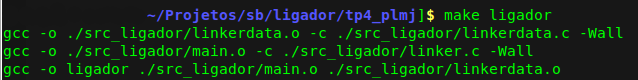
\includegraphics[scale=0.5]{./img/make.png}
 \caption{Comando Make}
\end{figure}

\begin{figure}[h!]
\centering
 
\includegraphics[scale=0.5]{./img/exec.png}
   \caption{Comando de execução do programa}
\end{figure}

\begin{figure}[h!]
\centering
 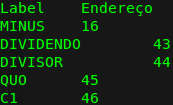
\includegraphics[scale=0.5]{./img/teste.png}
 \caption{saída usando verbose}
\end{figure}

\section{Conclusão}
\label{conclusao}
O trabalho correu sem grandes problemas, sendo a parte mais difícil a criação
dos progrmas de testes, pois montar alguns daqueles códigos em asembly é
extremamente difícil.

O programa atendeu a diversos valores de entrada e creio que a solução proposta
atenda ao especificado

\end{document}
